\documentclass[12pt, a4paper, oneside]{ctexart}
\usepackage{amsmath, amsthm, amssymb, bm, color, framed, graphicx, hyperref, mathrsfs, float}
\pagestyle{plain}
\usepackage{caption}
\captionsetup[figure]{labelsep=none}
\usepackage{tikz}

% multi-column
\usepackage{tasks}
% itemize
\NewTasksEnvironment[label=(\arabic*), label-width=3ex]{exercise}

\everymath{\displaystyle}

\title{\textbf{第三次作业}}
\author{U08M11002 Fall 2023}
\linespread{1}
\definecolor{shadecolor}{RGB}{241, 241, 255}

\newcounter{problemname}
\newenvironment{problem}{\stepcounter{problemname}\par\noindent\textbf{题目\arabic{problemname}. }}{\\\par}
\newenvironment{warning}{\begin{shaded}\par\noindent\textbf{提交作业方式:}}{\end{shaded}\par}

\begin{document}

\maketitle

\hspace{1em}

\begin{problem}
已知函数集$\cos t,\cos 2t,\cos 3t,....\cos nt,\sin t,\sin 2t,\sin 3t....\sin nt $ ($n \in \mathbb{Z}$)
\begin{exercise}(1)
	\task 试证明它是在时间区域[0,$2\pi$]内的正交函数集.
	\task 它是在时间区间[0,$2\pi$]内的完备正交函数集吗?
	\task 在时间区间[0,$\frac{\pi}{2}$]内,它是正交函数集吗?
\end{exercise}
\quad
\end{problem}

\begin{problem}
求下列两图中所示周期信号的傅里叶级数:
    \begin{figure}[H]
        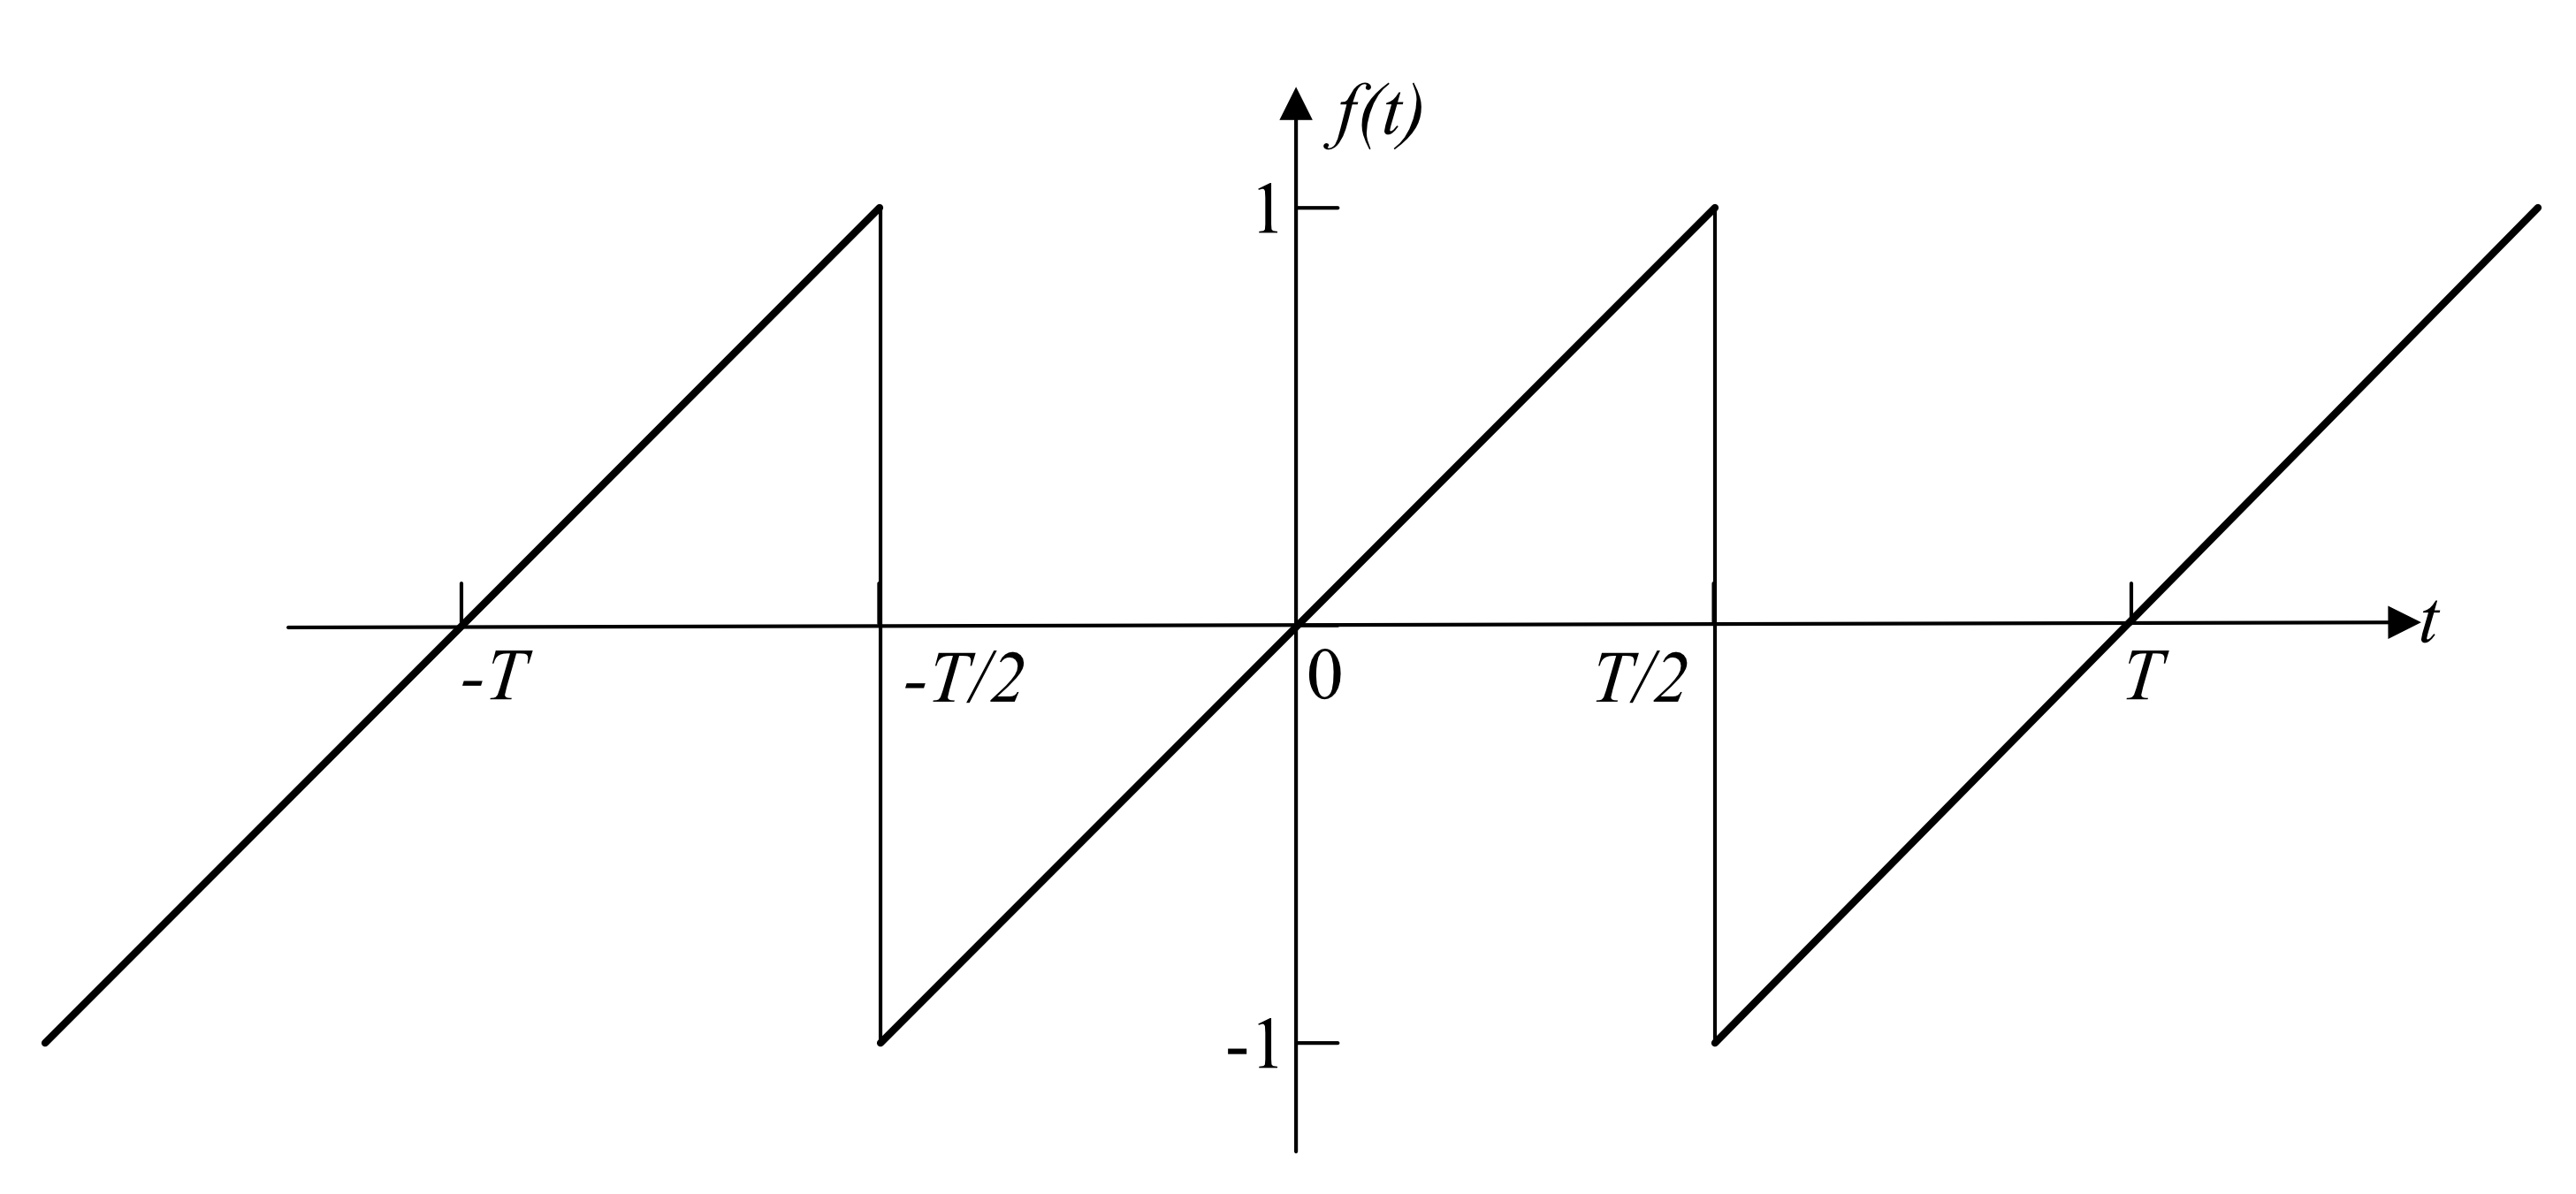
\includegraphics[width=12cm]{assets/hw4img1.png}
        \centering
        \caption*{(a)}
    \end{figure}
    \begin{figure}[H]
        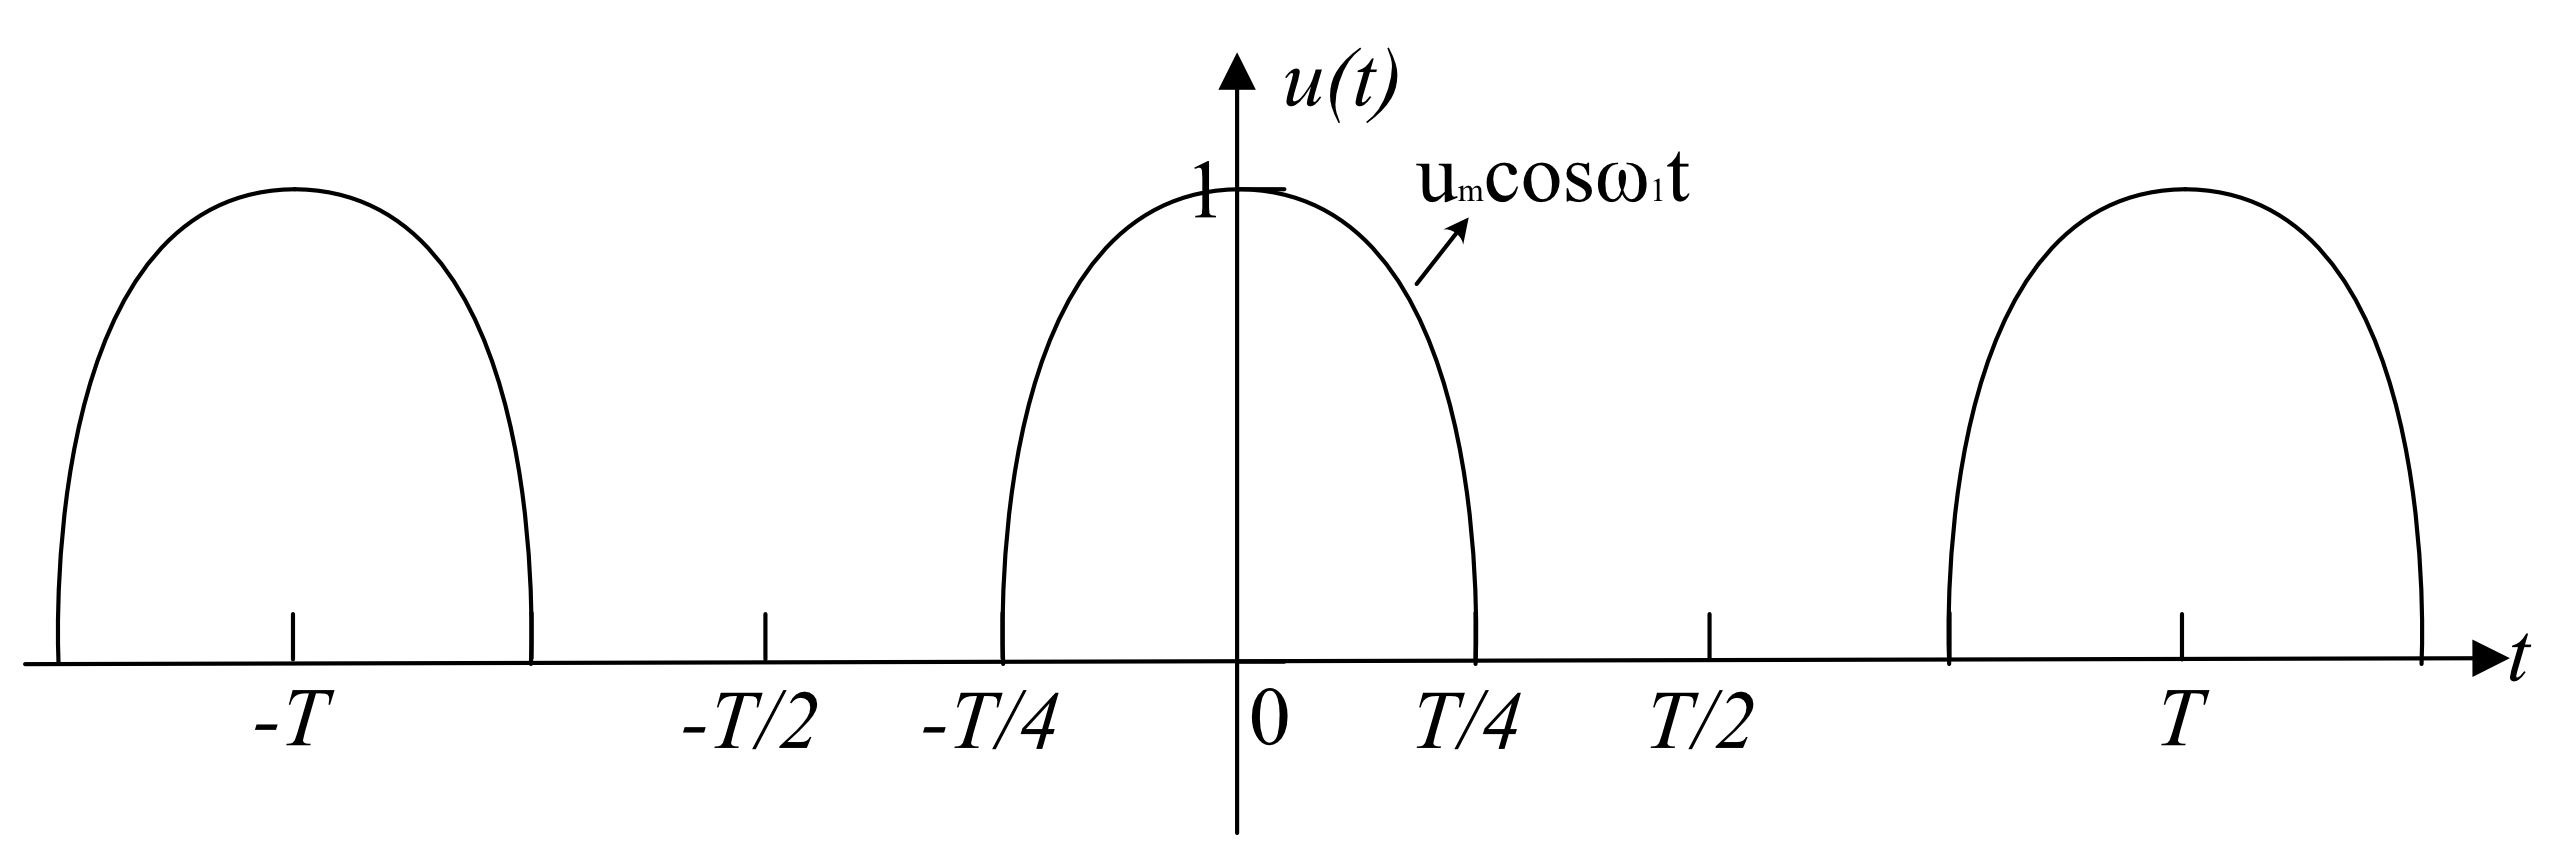
\includegraphics[width=12cm]{assets/hw4img2.png}
        \centering
        \caption*{(b)}
    \end{figure}
    
\quad
\end{problem}

\begin{problem}
已知单位冲激序列$\delta_T(t) = \sum_{k=-\infty}^{\infty}\delta(t-KT)$如下图所示.求其傅里叶级数与频谱。
	\begin{figure}[H]
		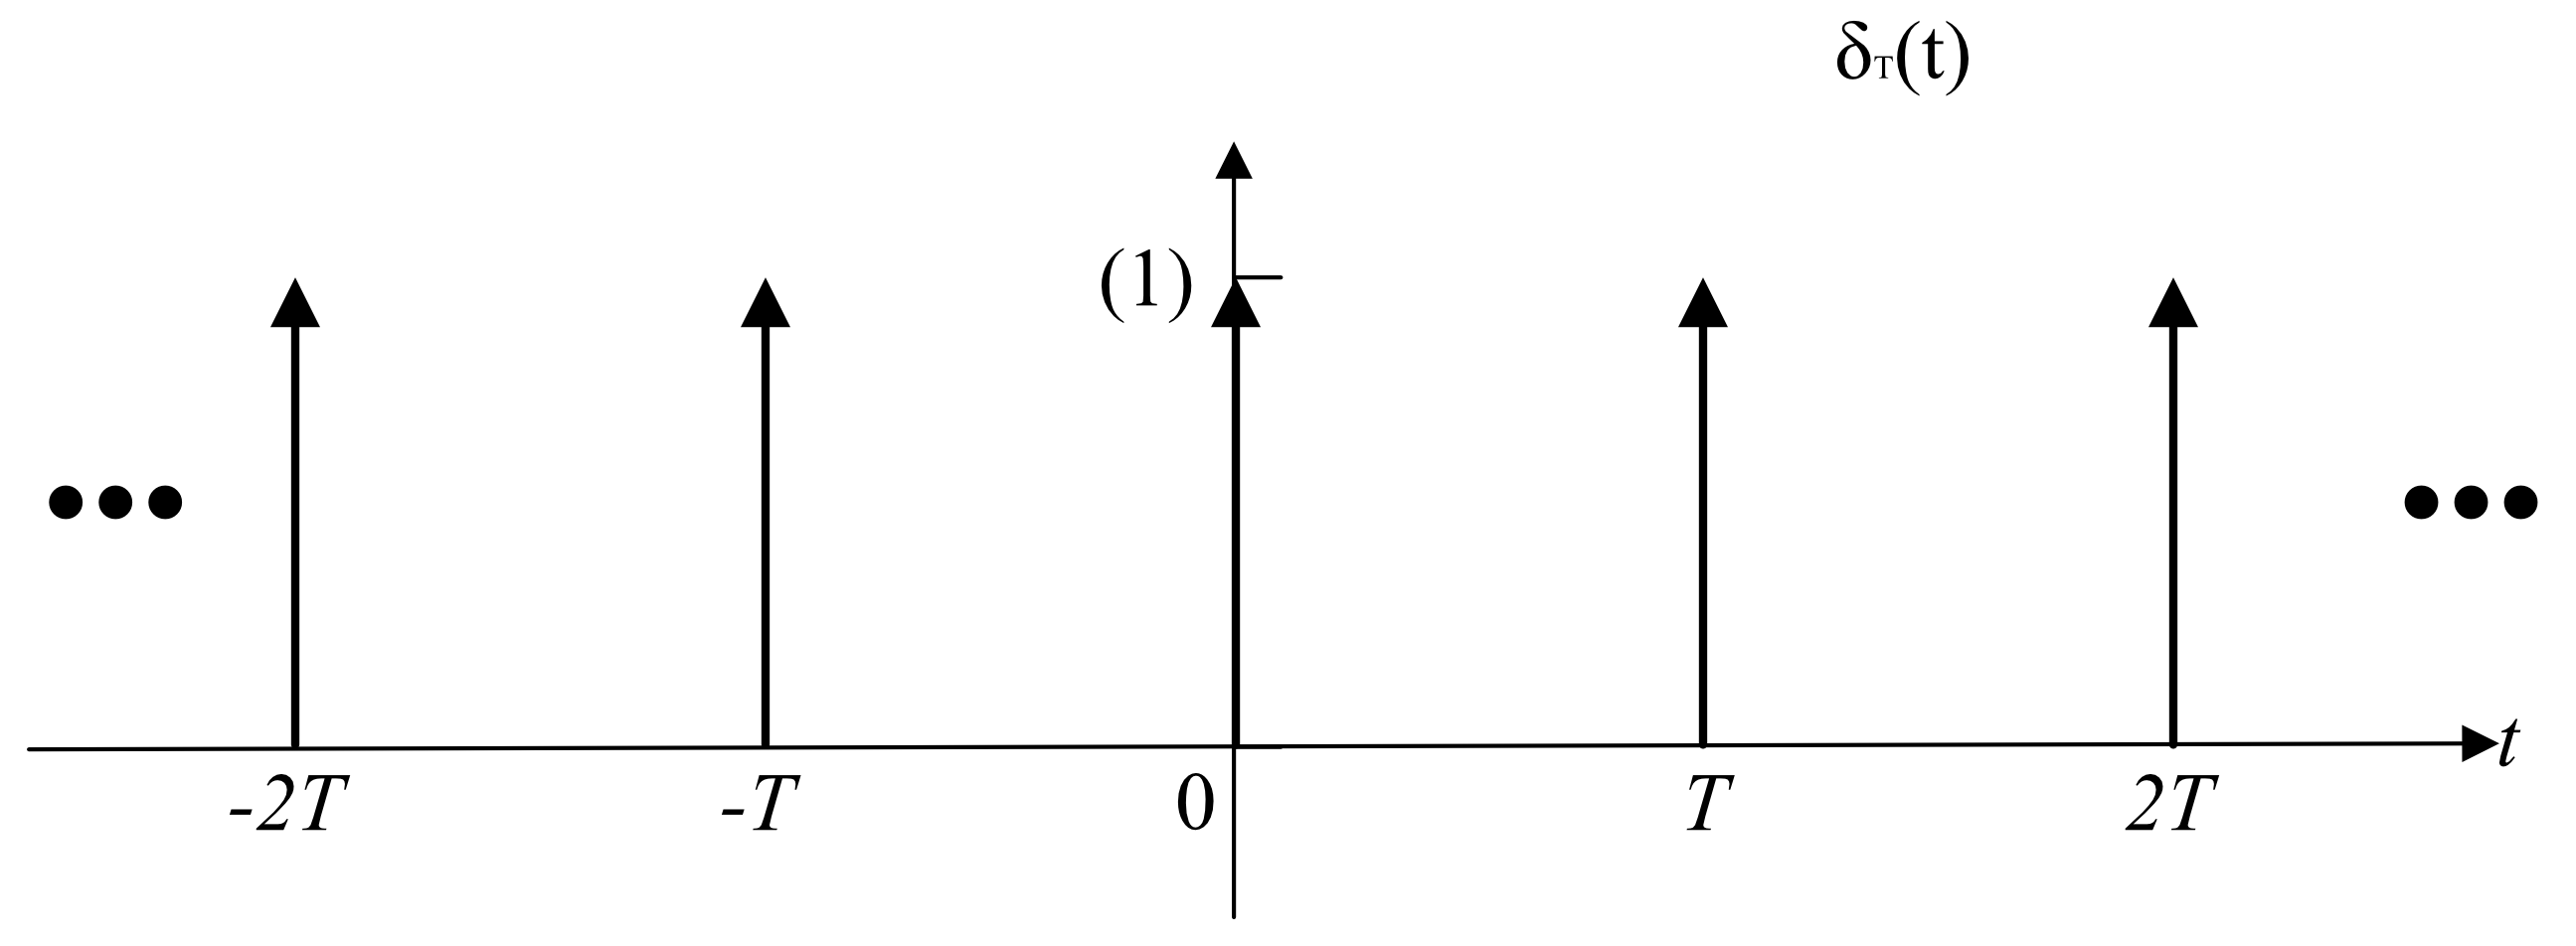
\includegraphics[width=12cm]{assets/hw4img3.png}
		\centering
	\end{figure}
\quad
\end{problem}

\begin{problem}
试画出下列周期信号$f(t)$的振幅频谱图和相位频谱图:
\begin{exercise}
	\task $f(t) = \frac{4}{\pi}[\cos(w_1t) -\frac{1}{3}\cos(3w_1t) + \frac{1}{5}\cos(5w_1t) - \frac{1}{7}\cos(7w_1t) + ....]$
	\task $f(t) = \frac{1}{2} - \frac{2}{\pi}[\sin(2\pi t) + \frac{1}{2}\sin(4\pi t) + \frac{1}{3}\sin(6\pi t) +....]$
\end{exercise}
\quad
\end{problem}

\begin{problem}
求下图所示两个信号的频谱函数。
	\begin{figure}[H]
		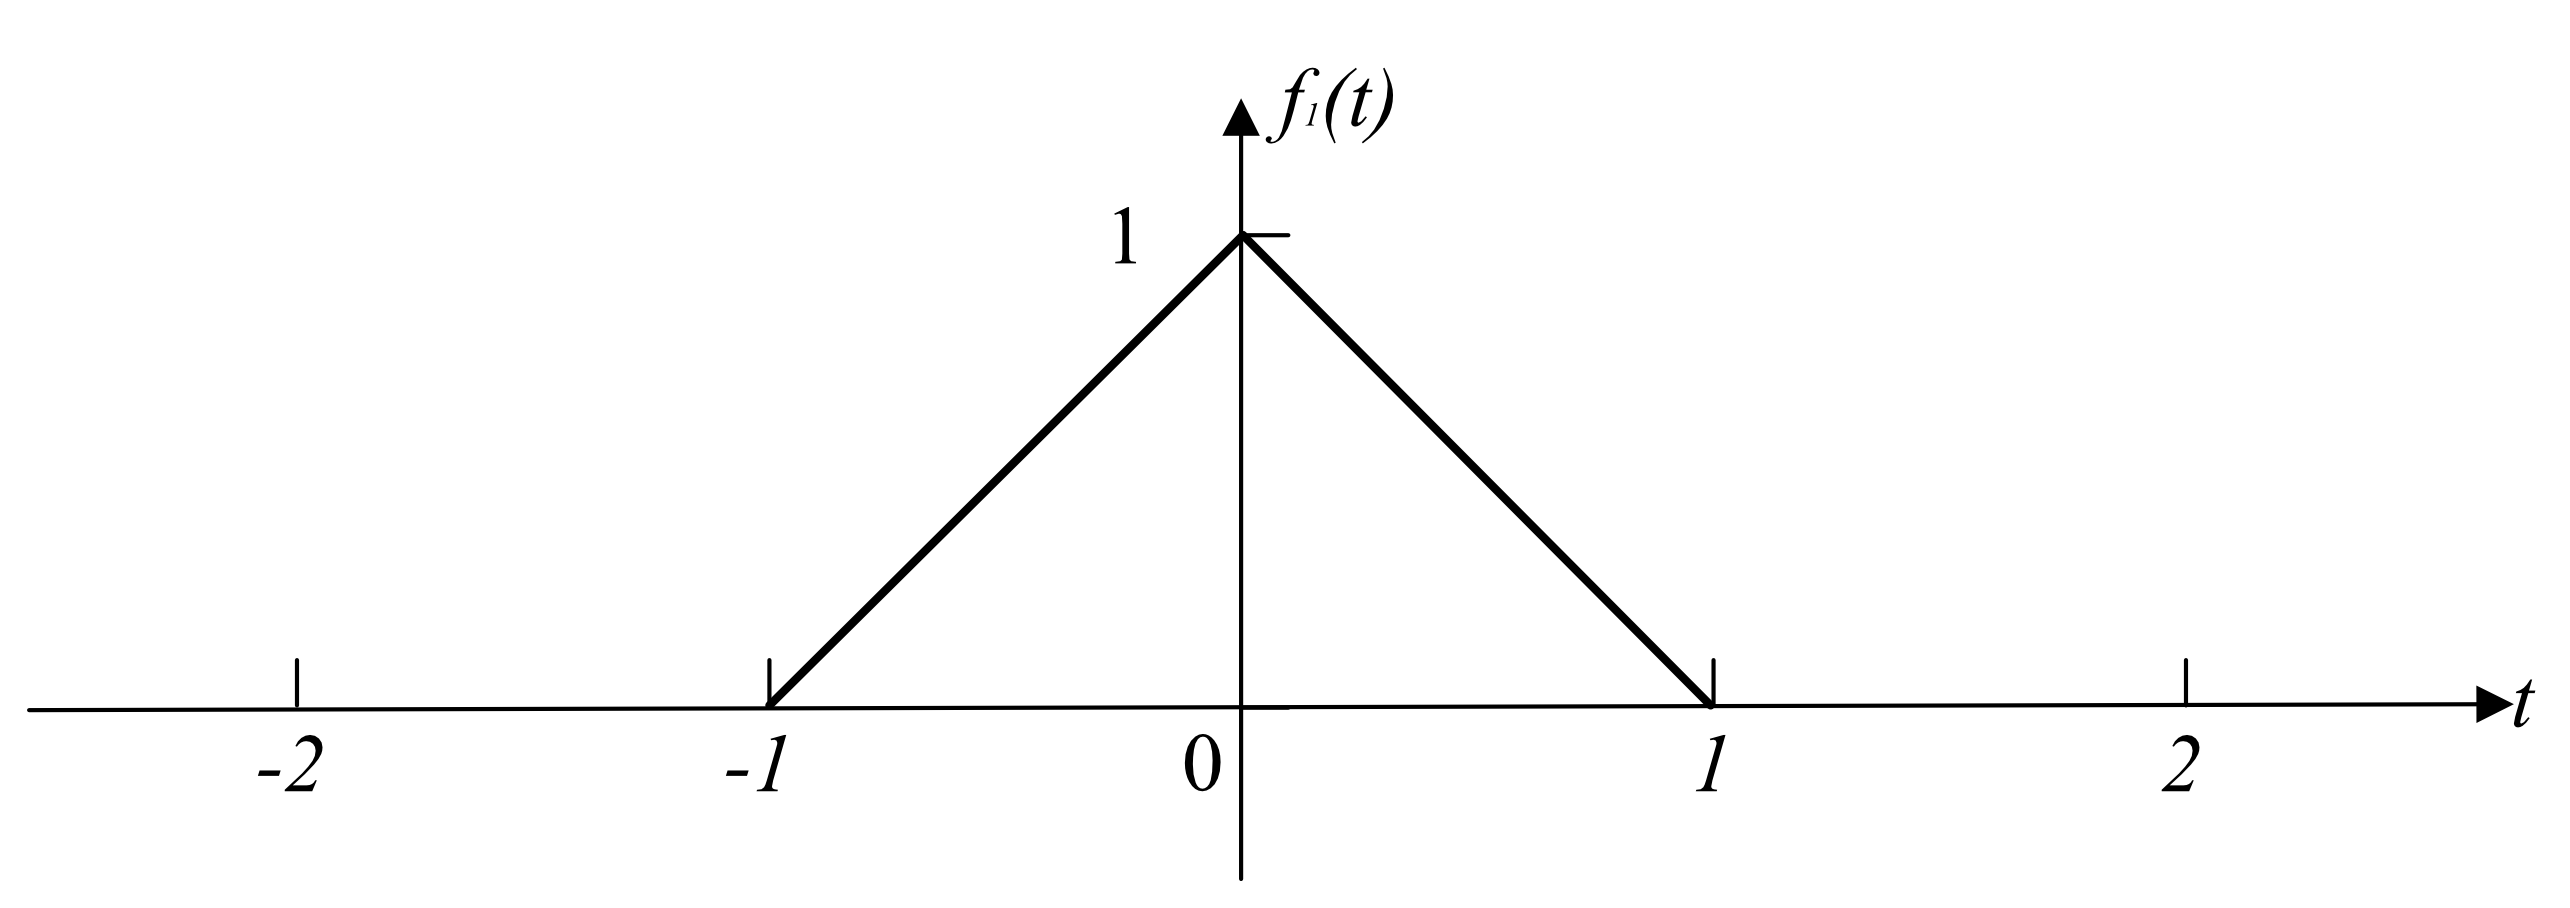
\includegraphics[width=12cm]{assets/hw4img4.png}
		\centering
        \caption*{(a)}
	\end{figure}
	\begin{figure}[H]
		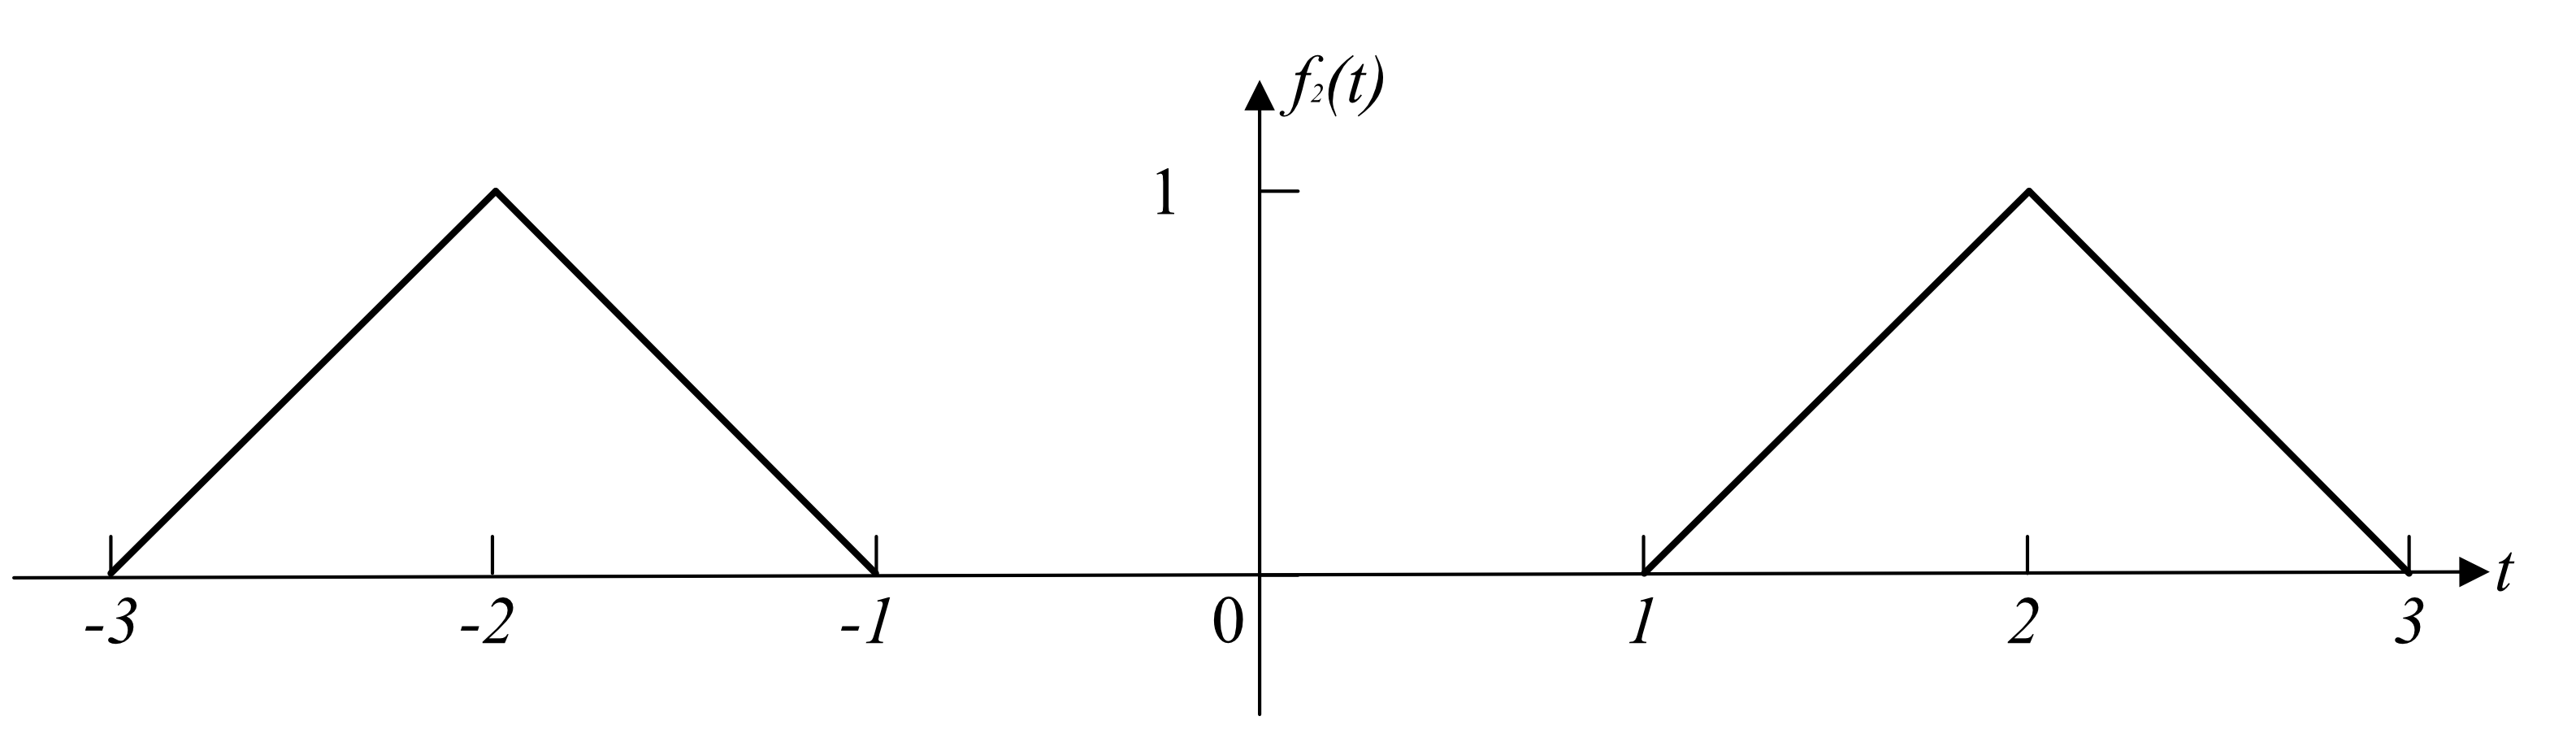
\includegraphics[width=12cm]{assets/hw4img5.png}
		\centering
        \caption*{(b)}
	\end{figure}
\quad
\end{problem}

\begin{problem}
求函数$f(t) = e^{-at}\epsilon(t)(a>0)$的自相关函数。
\quad
\end{problem}

\begin{problem}
求下列周期信号的基波角频率$\Omega$和周期T:
\begin{exercise}(2)
	\task $e^{j100t}$
	\task $\cos[\frac{\pi}{2}(t-3)]$
	\task $\cos(2t) + \sin(4t)$
	\task $\cos(2\pi t) + \cos(3\pi t) + \cos(5\pi t)$
	\task $\cos(\frac{\pi}{2}t) + \sin(\frac{\pi}{4}t)$
	\task $\cos(\frac{\pi}{2}t) + \cos(\frac{\pi}{3}t) + \cos(\frac{\pi}{5}t)$
\end{exercise}
\quad
\end{problem}

\begin{problem}
求下列信号的卷积:
\begin{exercise}
	\task 求图中 $f_1(t)$ 和 $f_2(t)$ 的卷积;
	\task $f_{1}(k) = \{\mathop{2}\limits_{\uparrow},2,1,-1 \}$,$f_{2}(k) = \{\mathop{0}\limits_{\uparrow},1,4,-2\}$;
	\task $f_1(k) = (0.5)^{k}U(k)$,$f_2(k) = U(-k)$;
\end{exercise}
\begin{figure}[H]
	\begin{center}
		\begin{tikzpicture}
			% 绘制 x 轴
			\draw[->] (-2,0) -- (2,0) node[right] {$t$};
			% 绘制 y 轴
			\draw[->] (0,-0.5) -- (0,1.5) node[above] {$f_1(t)$};
			
			% 绘制门函数
			\draw[line width=1pt] (-1,0) -- (-1,1) -- (1,1) -- (1,0);
			
			% 添加标签
			\node[below] at (-1,0) {-1};
			\node[below] at (1,0) {1};
			\node[left] at (0,1) {1};
		\end{tikzpicture}\
	\end{center}
	\caption*{(a)}
\end{figure}
\begin{figure}[H]
	\begin{center}
		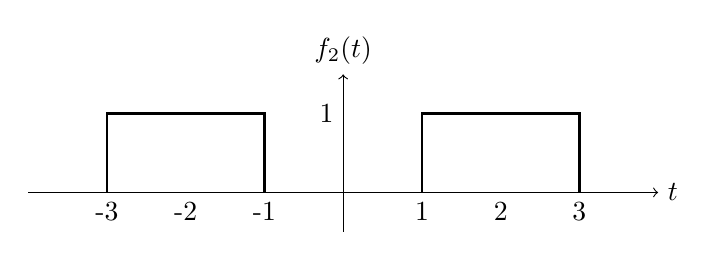
\begin{tikzpicture}
			% 绘制 x 轴
			\draw[->] (-4,0) -- (4,0) node[right] {$t$};
			% 绘制 y 轴
			\draw[->] (0,-0.5) -- (0,1.5) node[above] {$f_2(t)$};
			
			% 绘制门函数
			\draw[line width=1pt] (-3,0) -- (-3,1) -- (-1,1) -- (-1,0);
			\draw[line width=1pt] (3,0) -- (3,1) -- (1,1) -- (1,0);

			% 添加标签
			\node[below] at (-3,0) {-3};
			\node[below] at (-2,0) {-2};
			\node[below] at (-1,0) {-1};
			\node[below] at (1,0) {1};
			\node[below] at (2,0) {2};
			\node[below] at (3,0) {3};
			\node[left] at (0,1) {1};
		\end{tikzpicture}\
	\end{center}
	\caption*{(b)}
\end{figure}
\quad
\end{problem}

\begin{problem}
$f_1[k] = 3e^{-2t}U[k]$, $f_2[k] = 2U[k]$, $f_3[k] = 2U[k-2]$,求
\begin{exercise}(2)
	\task $f_1[k] * f_2[k] $
	\task $f_1[k] * f_3[k] $
	\task $f_2[k] * f_3[k] $
\end{exercise}
\quad
\end{problem}

\end{document}